\subsubsection{Availability Zone Usage}
\label{cloud-measure-zone}


Within each region of EC2, cloud tenants have the choice of deploying
across multiple zones. EC2 zones offer a means for improving service
robustness as they are claimed to use separate compute, network, and
power infrastructure so that a failure in any of these will not affect
more than one zone. There seems to be no
equivalent of zones in Azure.

We now focus on determining the zone deployment for
EC2-using services' front ends. Unlike the regions, which are easily
distinguished based on the IP address of a subdomain and the
advertised ranges~\cite{ec2iprange,azureiprange}, there is no direct way to associate an IP address
to a zone.  We therefore turn to cloud cartography
techniques~\cite{ristenpart2009hey}. We use two methods to identify
zones: network latency and proximity in the internal addresses to
instances with a known zone (i.e., VMs we launched).
Details about the two methods are presented in~\cite{he2013next}.
We combine the two zone identification methods to maximize the fraction of
physical instances whose zone we can identify.  We give preference to our
address-proximity-based zone identifications, and use our latency-based
identifications only for instances whose zone cannot be identified
using the former method.  Combining the two methods allows us to identify the
EC2 availability zone for 87.0\% of all physical EC2 instances in the
\alexadata dataset.

%\setlength{\tabcolsep}{0.1cm}
\begin{table}[t]
\center
\small
\begin{tabular}{|l||r|r|r|r|r|r|r|}
\hline
\bf Region & \multicolumn{2}{|c|}{1$^\textbf {st}$ \bf zone} &   \multicolumn{2}{|c|}{2$^\textbf {nd}$ \bf zone}   & \multicolumn{2}{|c|}{3$^\textbf {rd}$ \bf zone}  \\
           &\#Dom& \#Sub  & \#Dom& \#Sub & \#Dom& \#Sub\\
\hline
\awseast &  16.1  &  419.0&  6.2  & 155.4& 9.5  &  292.9 \\
\awscali &  1.6 &  33.2&  3.0  &  37.4 & N/A  &  N/A\\
\awsoreg  &  0.9 &  13.4 & 1.0 &  9.6 &0.8 &  7.3 \\
\awseuro  &   2.3  &  77.0&  2.9 & 63.9 & 4.5  &  98.7\\
\awstokyo &   0.4 & 3.7 & 1.3 & 11.3   &1.5 & 12.9 \\
\awssing  &  0.9 & 11.3 &   1.2 & 19.1 & N/A & N/A\\
\awssyd  &  0.2 & 0.3 & 0.2 & 0.3  & N/A & N/A \\
\awssp   &  0.5 & 14.4 &  0.2 & 8.9 & N/A & N/A\\
\hline
\end{tabular}
\caption{Estimated number of domains and subdomains using various EC2  zones. 
Some regions only have 2 zones.}
%Note there are only two zones in \awscali, \awssing, \awssyd and \awssp; there are three zones in \awstokyo, but we can only set up instances in two of them from Feb, 2013}
\label{tab:ec2-zone-usage}
\end{table}


\begin{figure}[!tb]
\centering
	\begin{subfigure}[b]{0.4\textwidth}
                \centering
                \includegraphics[width=\textwidth]{./figures/cloudmeasure/imag_sec4/zone_cdf_new_fix.pdf}
		\caption{subdomain}
		\label{fig:cloud_zone_subdomains_CDF}
	\end{subfigure}
	\begin{subfigure}[b]{0.4\textwidth}
                \centering
                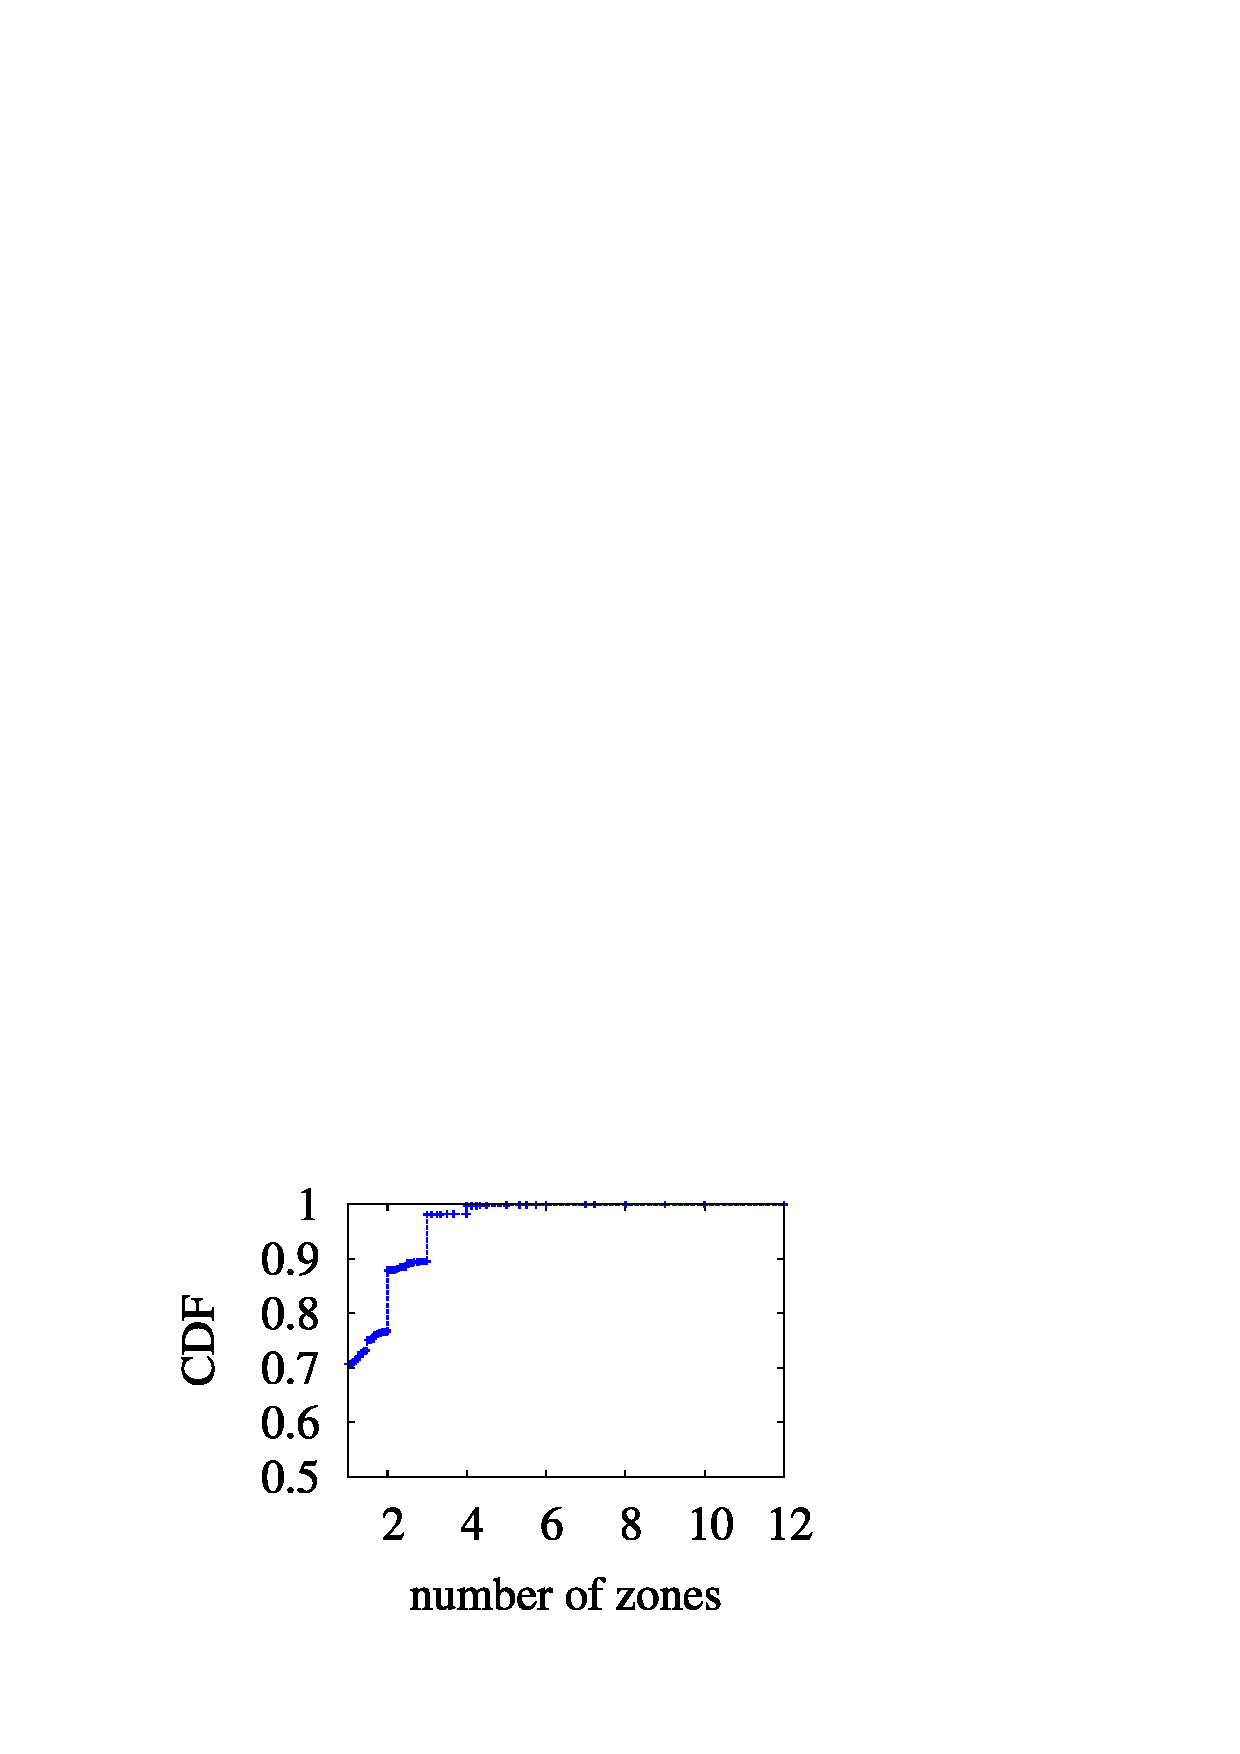
\includegraphics[width=\textwidth]{./figures/cloudmeasure/imag_sec4/avg_zone_cdf_new_fix.pdf}
		\caption{domain}
		\label{fig:cloud_zone_domains_CDF}
	\end{subfigure}
\caption{(a) CDF of the number of zones used by each subdomain 
(b) CDF of the average number of zones used by the subdomains of each domain.}
\label{fig:cloud_zone_CDF}
\end{figure}

\begin{table}[t]
\centering
\small
\input{cloudmeasure_tables/tab_domain_deploy_zone.tex}
\caption{Zone usage estimates for top using zones. Column 4 is estimated 
total number of zones used by all
subdomains. Columns 4--6 indicate the estimated number of subdomains that use 
$k$ different zones.}
\label{top_alexa_domains_deploy_zone}
\end{table}


\tabref{tab:ec2-zone-usage} summarizes the number of (sub)domains using each region and
zone.  In all but one region (Asia Pacific Southeast 2), we
observe a skew in the number of subdomains using each zone in a region. Asia
Pacific Northeast and US East regions have the highest skew across their
three zones: 71\% and 63\% fewer subdomains, respectively, use the least
popular zone in those regions compared to the most popular zone.  

We also look at the number of zones used by each (sub)do-main.
\figref{fig:cloud_zone_subdomains_CDF} shows a CDF of the number of
zones used by each subdomain.  We observe that 33.2\% of
subdomains use only one zone, 44.5\% of subdomains use two zones, and 22.3\%
of subdomains use three or more zones.  Of the subdomains that use two or
more zones, only 3.1\% use zones in more than one region.  
%For example, if
%the one of the zones in the US East region failed, \fixme{XX\%, XX\%, and
%XX\%} of subdomains would be completely unavailable if the 1st, 2nd, or 3rd
%zones, respectively, failed.
\figref{fig:cloud_zone_domains_CDF} shows the average number of zones used by
the subdomains of each domain.  We observe that most domains (70\%) only use
one zone for all subdomains; only 12\% of domains use two or more zones per
subdomain on average.  

Even for the top EC2-using domains, a large fraction of their subdomains only
use a single zone (\tabref{top_alexa_domains_deploy_zone}). For example,
56\% of pinterest.com's EC2-using subdomains and 33\% of linkedin.com's are
only deployed in one zone.  

%\figref{az_num} breakdowns the number of availability zones deployed by
%EC2-using subdomains by region.

\tightparagraph{Summary and implications} Our two key findings in this section
are that ({\em i}) the majority of EC2-using subdomains only use one (33.2\%)
or two (44.5\%) zones, and ({\em ii}) the subdomains using a given EC2 region
are not evenly spread across the availability zones in that region. The former
implies that many EC2-using subdomains would be completely unavailable if a
single zone failed, and many others would be severely crippled: e.g., a
failure of \awseasta would cause 16.1\% of subdomains to be completely
unavailable.  Our later key finding implies that an outage of a particular
zone in a region may have a greater negative impact than an outage of a
different zone in the same region: e.g., a failure of \awseasta would impact
$\approx$419K subdomains, while a failure of \awseastb would only impact
$\approx$155K.



